\documentclass{article}
%\documentclass{scrartcl}
\usepackage[utf8]{inputenc}
\usepackage[a4paper,top=2cm,bottom=2cm,left=3cm,right=3cm,marginparwidth=1.75cm]{geometry}
\usepackage{amsmath}
\usepackage{amssymb}
\usepackage{graphicx}
\usepackage[colorlinks=true, allcolors=blue]{hyperref}
\usepackage{float}
\usepackage{caption}
\captionsetup{justification=centering}
\usepackage{subcaption}
\usepackage{hyperref}
\usepackage[font=small,labelfont=bf,justification=justified]{caption}
\usepackage[utf8]{inputenc}
\usepackage[backend=biber, style=authoryear]{biblatex}
\addbibresource{references.bib}  % your .bib filename here
\setcounter{secnumdepth}{4}
\renewcommand{\theparagraph}{\thesubsubsection.\alph{paragraph}}
\usepackage{verbatim}

\begin{document}
	
	\begin{titlepage}
		\centering
		\vspace{0.5em}
		
		{\scshape\LARGE Université Paris Cité \par}
		\vspace{0.4cm}
		{\large Département de mathématiques et d'informatique}
		
		\vspace{1cm}  
		
		{\Large \bfseries Influence du type phytoplanctonique et des structures de méso échelle sur la distribution des organismes mésopélagiques\par}
		\vspace{0.2cm}
		{\Large  Rapport de stage\par}
		
		\vspace{1cm}
		
		\begin{abstract}
			
		\end{abstract}
		
		\vspace{1cm}
		
		{\large \textbf{Rapport réalisé par}}\\[0.2cm]
		{\large Elise NICOLAS\par}
		
		\vspace{0.6cm}
		
		{\large \textbf{Encadrants}}\\[0.2cm]
		{\large Marius MOLINET, David NERINI, Christophe GUINET, Cédric COTTET}
		
		\vspace{0.6cm}
		
		{\large \textbf{Professeure référente}}\\[0.2cm]
		{\large FISHER Aurélie}
		
		
		
		\vspace{0.8cm} 
		
		{\large \date{} \par}
	\end{titlepage}
	
	%------------------------------------
	\clearpage
	\tableofcontents
	
	%------------------------------------
	\clearpage
	\section{Introduction}
	L'océan couvre 70\% de la surface terrestre. La répartition des terres émergés n'est pas équivalente selon les deux hémisphères: l'hémisphère Sud est composé à 80.9\% de mer, contre 60.7\% pour l'hémisphère Nord. Dans l'hémisphère Sud, dans le bassin Antarctique, les océans Atlantique, Pacifique et Indien se connectent. Une seul masse d'eau liquide se déplace alors dans les différents bassins. L'océan planétaire est un milieu continu. 
	\begin{figure}[h]
		\center
		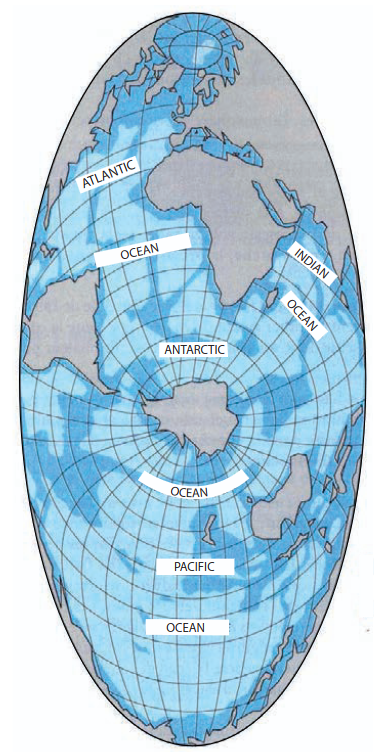
\includegraphics[width=0.3\textwidth]{images/intro/continuity_planteraryocean_fieux}
		\caption{Représentation des différents bassins océaniques et de leurs continuité.}
		\label{oceans}
	\end{figure}
	
	Un biotope correspond à l'espace physique et les conditions abiotiques associées dans lesquelles vit une biocénose. Une biocénose est l'ensemble des populations d'organismes qui occupent une zone donnée et interagissent entre elles. L'océan étant un milieu continu, seuls les paramètres physiques de l'eau (abiotiques) conditionnent la régionalisation en biotopes. La connaissance des paramètres physiques de l'eau est donc particulièrement importante pour l'étude des distribution des organismes et des niches écologiques marines. Les principaux paramètres abiotiques structurant les écosystèmes sont : la lumière (longueur d'onde et proportion d'éclairement), les propriétés hydrologiques (température et salinité) et l'hydrodynamisme. \textbf{il faut une source}. L'océan est stratifié verticalement selon la pénétration de la lumière : celle-ci dépendant de la profondeur. On parle de milieu eutrophe (épipélagique) entre 0 et 200m, de milieu dysphotique (mésopélagique) entre 200 et 1000m, de milieu aphotique (bathypélagique) entre 1000 et 4000m et de milieu abyssal au delà de cette dernière. Les propriétés hydrologiques de l'eau dépendent du climat : la chaleur et le vent induisent une évaporation rendant l'eau de mer plus salée, les précipitations induisent un adoucissement de la salinité. La composition chimique de l'eau de mer est fortement dépendante des apports du littoral (fer, nitrates, etc). L'hydrodynamisme inclue les marées et les divers courants induits par des gradients de température, de pressions. Ces derniers dépendent majoritairement du vent et de l'ensoleillement. La proximité au littoral participant grandement à la modification de ces paramètres abiotiques, on sépare l'océan horizontalement selon sa distance au plateau continental. On parle de zone pélagique au delà du plateau continental.
	
	L'écologie est une discipline qui s'intéresse aux interactions entre les différentes espèces d'un même biotope. Parmi elles, les relations trophiques (alimentaires) jouent un rôle fondamentale dans la structuration des écosystèmes. Dans le milieu océanique, le réseau trophique peut généralement être simplifié comme suis : 
	\begin{itemize} 	
		\item les producteurs primaires sont le phytoplancton
	\end{itemize}
	
	
	
	\subsection{L'Océan Austral}
	L'océan Austral (ou Antarctique) forme un anneau autour de l'Antarctide. Il représente 22\% de la surface totale des océans. Contrairement aux autres océans, iln'est pas délimité par des frontières continentales. En regardant une carte (voir figure \ref{label}), on pourrait penser qu'il est simplement la prolongation du bassin Atlantique, Pacifique et Indien. En réalité, il est délimité par une frontière océanographique : le Front Subtropical (approximativement à 40°S), caractérisé par de très forts gradients de températures. L'océan Austral se distingue également des autres océans par l'uniformité de son climat, de son hydrodynamisme et de ses propriétés hydrologiques.
	
	
	\subsection{Contexte Biologique}
	\subsubsection{Stratification Verticale}
	\subsubsection{Réseau Trophique}
	% plancton nekton etc
	
	
	\subsection{Contexte Physique}
	\subsubsection{}
	%------------------------------------
	\clearpage
	\section{Matériel}
	% schema de toutes les donnnées
	\subsection{Données issue de campagnes océanographiques/in situ (Marion Dufresnes II)}
	\subsection{Données Environnementales}
	
	%------------------------------------
	\clearpage
	\section{Méthode}
	% schéma de la pipeline
	\subsection{Pré-traitement des données}
	\subsubsection{Gestion des valeurs manquantes}
	% cropper les données et couper au dessus
	
	\subsubsection{Estimation semi-paramétrique des profils d'intensité de rétropropagation $Sv$}
	\paragraph{Motivation}
	Les profils d'intensité de rétropropagation $Sv \in \mathbb{R}^{n_{freqs} \times n_{pings} \times n_{depths}}$, $Sv_{l, i} \in \mathbb{R}^{n_{depths}}$ issus des campagnes océanographique sont bruités et fortement irréguliers : $Sv_{l, i} = x_{l,i}(t) + \epsilon_{i}$. 
	Afin de faciliter l'étude de ces profils (gestion de valeurs manquantes, dérivations, étude sur des grilles différentes, FPCA, \textit{etc}), on estime la fonction $x_i (t_j) : \tau \rightarrow \mathbb{R}$ par projection sur des bases de B-splines.
	
	\begin{comment}
		\paragraph{Espaces de Sobolev $\mathcal{H}^{2}$}
		De par ses propriétés de continuité, l'espace $\mathcal{H}^{2}(\tau)$ est un cadre naturel pour estimer $x_{l, i}$. \\
		
		Soit $ \tau = [a, b] \subset \mathbb{R}$ un intervalle borné. L'espace de Sobolev $\mathcal{H}^{2}(\tau)$ est définit par : 
		\begin{equation}
			\mathcal{H}^{2}(\tau) = \{f \in \mathcal{L}^{2}(\tau)|f', f'' \in \mathcal{L}^{2}(\tau) \}
			\label{h2}
		\end{equation}
		
		avec $f'$ et $f''$ les dérivées entendues au sens faible.\\
		
		\vspace{0.2em}
		Il est munit du produit scalaire 
		\begin{equation}
			<f, g>_{H^{2}} = \int_\tau f(t) g(t) dt + \int_\tau f'(t) g'(t) dt + \int_\tau f''(t) g''(t) dt
			\label{norme_h2}
		\end{equation}
		
		et de la norme induite $||f, g||_{H^{2}} = \sqrt{<f, g>_{H^{2}}}$. \\
		
		\vspace{0.2em}
		
		\textbf{Propriété clé des espaces de Sobolev}
		Par le théorème de plongement de Sobolev en dimension 1, toute fonction $f \in \mathcal{H^{2}}(\tau) \in \mathcal{C}^{1}$, est continûment différentiable. Cette propriété est particulièrement importante pour l'estimation par moindre carrés pénalisée comme on le verra dans le paragraphe \ref{par:moindres_carres}.
		
	\end{comment}
	
	\paragraph{B-splines d'ordre $k$ (\cite{deBoor})}
	Les B-splines sont des fonctions pouvant servir de base pour l'estimation fonctionelle (B pour "Basis"). Ce sont des polynômes par morceaux pourvus de certaines conditions de régularités aux noeuds (ou points de rupture). La Figure \ref{fig:bsplines} montre un exemple simple de B-splines (\cite{eilers1996}) : en (a) est montrée une B-spline de degré 1 et en (b) une B-spline de degré 2. 
	\begin{figure}[h]
		\centering
		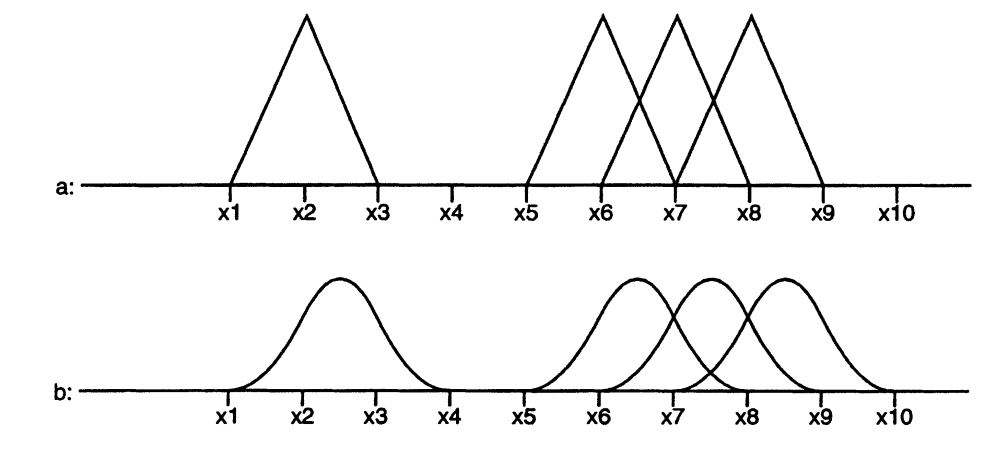
\includegraphics[width=0.6\textwidth]{images/methodology/b_splines_eilers}
		\caption{Illustration d'une B-spline isolée de B-splines chevauchantes, de degré 1 (a) et de degré 2 (b) (\cite{eilers1996})}
		\label{fig:bsplineseilers}
	\end{figure}
	
	
	Soit $\tau_i, \ldots, \tau_{i+m+1}$ noeuds (équi-espacés ou non) avec $m$ le degré de la B-spline (on a donc un ordre valant $m+1$) 
	
	Soit $\phi_{i,m}(x)$ la B-spline d'ordre $m$ dont le support est $supp(\phi(x)) = [\tau_i, \tau_{i+m+1}]$. On peut définir la B-spline $\phi_{i,m}(x)$ par la formule de réccurence de Cox-de-Boor (\cite{deBoor}) : 
	\begin{enumerate}
		\item \textbf{Initialisation d'une fonction porte par noeud (ordre 1)}
		\begin{equation}
			\phi_{i,1} = \begin{cases}
				1 & \text{si } \tau_i \leq x < \tau_{i+1} \\
				0 & \text{sinon}
			\end{cases}
		\end{equation}
		
		\item \textbf{Réccurence : combinaison convexe de la B-spline d'ordre inférieur à différents noeuds}
		\begin{equation}
			\phi_{i, m} = \omega_{i,m}(x) \phi_{i, m-1} + (1 - \omega_{i,m}(x)) \phi_{i+1, m-1}
		\end{equation}
		avec 
		\begin{equation}
			\omega_{i,m}(x) := \frac{x - \tau_i}{\tau_{i+m-1}- \tau_i}
		\end{equation}
	\end{enumerate}
	
	\textbf{Propriétés des B-Splines de degré $m$ : Support, positivité et régularité}
	La B-spline $\phi_{i, m}(x)$ est un polynôme par morceau de degré $m$ (et d'ordre $m+1$) avec des points de rupture (noeuds) $\tau_i, \ldots, \tau_{i+m} $ à les propriétés suivantes :
	\begin{itemize}
		\item Continuité : $\phi_{i, m}(x) \in C^{m-1}$ au noeuds (les dérivées jusqu'a l'ordre m-1 sont continues sur les noeuds). Pour une B-spline cubique ($m=3$), $\phi_{i, 3} \in \mathcal{C}^{2}$,
		\item Support compact : $\text{supp}(\phi_{i,m}) = [\tau_i, \tau_{i+m+1}]$, 
		donc $\langle \phi_{i,m}, \phi_{j,m} \rangle = 0$ si $|i-j| \geq m+1$.
		\item Positivité : $\phi_{i,m}(x) > 0$ sur $(\tau_i, \tau_{i+m+1})$ 
		et $\phi_{i,m}(x) = 0$ sinon.
	\end{itemize}
	
	
	\paragraph{Espace des splines $\mathbb{S}_{m, \tau}$}
	Une fonction spline $f : [a, b] \rightarrow \mathbb{R}, f\in \mathbb{S}_{m, \tau}$ de degré $m$ avec suite de noeuds $\tau$ est toute combinaison linéaire de B-splines de degré $m$ pour la suite de noeuds $\tau$. 
	La suite de noeuds $\tau$ est la suivante : 
	\begin{equation}
		\underbrace{a = \tau_1 = \tau_2 = \cdots = \tau_{m+1}}_{m+1 \text{ noeuds répétés en } a} 
		< 
		\underbrace{\tau_{m+2} < \cdots < \tau_{m+L+1}}_{L \text{ noeuds intérieurs}} 
		< 
		\underbrace{\tau_{m+L+1} = \cdots = \tau_{2\times L+m+1}=b}_{m+1 \text{ noeuds répétés en } b}
	\end{equation}
	
	La collection de toutes ces fonctions est notée $\mathbb{S}_{m,\tau}$. Les B-splines $\{\phi_{i,m}\}_{i=0}^{m+L+1}$ forment alors une base de cet espace de dimension $\dim(\mathbb{S}_{m,\tau}) = L + m + 1$, avec $L$ le nombre de noeuds intérieurs.. 
	
	\begin{equation}
		\mathbb{S}_{m,\tau} := \left\{ \sum_{i=1}^{L+m+1} \alpha_i \phi_{i,m} \;:\; \alpha_i \in \mathbb{R}\right\}
	\end{equation}
	
	\paragraph{Estimation fonctionnelle par minimisation des moindres carrés 
		pénalisée (O-Splines) (\cite{wand2008}, \cite{eilers1996})}
	\label{par:moindres_carres}
	
	Considérons une régression non-paramétrique simple :
	\begin{equation}
		y_k = f(x_k) + \varepsilon_k, \quad \forall k \in \{1, \ldots, n\}
	\end{equation}
	
	où $(x_k, y_k) \in \mathbb{R} \times \mathbb{R}$ et $n$ le nombre de données.
	
	Supposons qu'une estimation de $f$ est nécessaire sur $[a, b]$, un intervalle 
	contenant les $x_i$. Soit $\hat y : [a, b] \rightarrow \mathbb{R}, f \in \mathbb{S}_{m, \tau}$ une spline (combinaison linéaire de B-splines de degré m) estimée de f :
	\begin{equation}
		\hat y(x_k) = \sum_{i=1}^{m+L+1} \alpha_i \phi_{i,m}(x_k),
	\end{equation}
	où $\phi_1, \ldots, \phi_{m+L+1}$ sont les B-splines de degré $m$, et $L$ le nombre de noeuds intérieurs, avec $\text{supp}(\phi_{i,m}) = [\tau_i, \tau_{i+m}]$.
	
	La fonction objective des moindres carrés (MSE pour "\textit{Mean Square Error}" à minimiser est :
	\begin{align}
		S &= \sum_{k=1}^{n} \left(y_k - \hat{f}(x_k)\right)^{2} \\
		&= \sum_{k=1}^{n} \left(y_k - \sum_{i=1}^{L+m+1} 
		\alpha_i\, \phi_{i,m}(x_k)\right)^{2}
	\end{align}
	
	Choisir le nombre de nœuds $K = m+L$ des B-splines peut s'avérer difficile, et peut induire de l'overfitting (un grand nombre de nœuds permet de capturer toutes les variations des données d'entraînements mais donne de mauvaises performances de régressions sur des nouvelles données tests, les données tests étant différentes des données d'entraînement). Plusieurs techniques de pénalisation (Paul H. C. Eilers, Brian D. Marx, O'Sullivan) ont été mises en place pour choisir les hyper-paramètres des B-splines (nombre de nœuds) de manière optimale. On présentera ici la régression pénalisée de O'Sullivan (1986). Se référer aux travaux de (\cite{wand2008}, \cite{eilers1996}) pour d'avantages de détails sur les autres méthodes.\\
	
	La régression de O'Sullivan pénalise la rugosité de la fonction estimée, c'est à dire à quel point elle oscille ou est irrégulière.
	
	Le terme de pénalisation de O'Sullivan (matrice de rugosité) ajouté à la MSE (Mean Square Error) est définie par :
	\begin{equation}
		\Omega_{i,j} = \int_{a}^{b} \phi_{i,m}''(x)\, \phi_{j,m}''(x)\, dx, 
		\quad 1 \leq i, j \leq K
	\end{equation}
	
	La MSE pénalisée (O-Sullivan, Ridge fonctionnel) est alors :
	\begin{equation}
		S_\lambda = \underbrace{\sum_{k=1}^{n} \left(y_k - \sum_{i=1}^{K} 
			\alpha_i\, \phi_{i,m}(x_k)\right)^{2}}_{\text{MSE}} 
		+ \lambda \underbrace{\boldsymbol{\alpha}^\top \Omega\, 
			\boldsymbol{\alpha}}_{\text{rugosité}}
	\end{equation}
	
	où $\lambda \geq 0$ est le paramètre de lissage contrôlant le compromis entre 
	fidélité aux données (MSE) et régularité de $\hat y$.\\
	
	\textbf{Forme matricielle.} En posant $\mathbf{y} = (y_1, \ldots, y_n)^\top$, 
	$\boldsymbol{\alpha} = (\alpha_1, \ldots, \alpha_K)^\top$ et la matrice de design 
	$\mathbf{\phi} \in \mathbb{R}^{n \times K}$ telle que $\mathbf{\phi}_{k,i} = \phi{i, m}(x_k)$, 
	on réécrit :
	\begin{equation}
		S_\lambda = \left(\mathbf{y} - \mathbf{\phi}\boldsymbol{\alpha}\right)^\top 
		\left(\mathbf{y} - \mathbf{\phi}\boldsymbol{\alpha}\right) 
		+ \lambda\, \boldsymbol{\alpha}^\top \Omega\, \boldsymbol{\alpha}
	\end{equation}
	
	\textbf{Solution analytique.} Puisque $S_{\lambda}$ est convexe en $\alpha$, on peut trouver les coefficients $\alpha$ minimaux en annulant la dérivée de $S_\lambda$ par rapport à 
	$\boldsymbol{\alpha}$ :
	\begin{equation}
		\frac{\partial S_\lambda}{\partial \boldsymbol{\alpha}} = 
		-2\mathbf{\phi}^\top(\mathbf{y} - \mathbf{\phi}\boldsymbol{\alpha}) 
		+ 2\lambda\, \Omega\, \boldsymbol{\alpha} = \mathbf{0}
	\end{equation}
	
	On obtient l'estimateur :
	\begin{equation}
		\hat{\boldsymbol{\alpha}} = \left(\mathbf{\phi}^\top \mathbf{\phi} + 
		\lambda\, \Omega\right)^{-1} \mathbf{\phi}^\top \mathbf{y}
	\end{equation}
	
	et les valeurs ajustées :
	\begin{equation}
		\hat{\mathbf{y}} = \mathbf{\phi}\hat{\boldsymbol{\alpha}} = 
		\underbrace{\mathbf{\phi}\left(\mathbf{\phi}^\top \mathbf{\phi} + 
			\lambda\, \Omega\right)^{-1} \mathbf{\phi}^\top}_{\mathbf{H}(\lambda)}\, \mathbf{y}
	\end{equation}
	
	où $\mathbf{H}(\lambda)$ est la \textit{matrice d'influence}, 
	similaire à la projection orthogonale de la régression linéaire classique.\\
	
	\textbf{Choix du paramètre de lissage $\lambda$ par validation croisée 
		leave-one-out (CV-LOO).} Le paramètre $\lambda$ contrôle la régularité de 
	la courbe estimée : un $\lambda$ trop petit conduit à de l'overfitting, 
	un $\lambda$ trop grand à de l'underfitting. La validation croisée 
	leave-one-out consiste à estimer l'erreur de prédiction en retirant tour 
	à tour chaque observation $i$ :
	\begin{equation}
		\text{CV}(\lambda) = \frac{1}{n}\sum_{i=1}^{n} 
		\left(y_i - \hat{f}^{(-i)}(x_i)\right)^{2}
	\end{equation}
	
	où $\hat{f}^{(-i)}$ est l'estimateur calculé sans l'observation $i$. 
	Grâce à la hat matrix $\mathbf{H}(\lambda)$, on dispose d'une formule 
	analytique évitant de refaire $n$ régressions :
	\begin{equation}
		\text{CV}(\lambda) = \frac{1}{n}\sum_{i=1}^{n} 
		\left(\frac{y_i - \hat{y}_i}{1 - H_{ii}(\lambda)}\right)^{2}
	\end{equation}
	
	où $H_{ii}(\lambda)$ est le $i$-ème élément diagonal de $\mathbf{H}(\lambda)$. 
	Le paramètre optimal est alors :
	\begin{equation}
		\hat{\lambda} = \underset{\lambda > 0}{\arg\min}\; \text{CV}(\lambda)
	\end{equation}
	
	Dans notre cas, le nombre d'observations étant très important, on se limite a une validation croisée sur un sous-ensemble d'observations.
	
	
	\subsection{Réduction de dimension par Functional Principal Component Analysis}
	
	l'Analyse par Composante Principale Fonctionelle (ACPF ou \textit{FPCA} pour Functional Principal Component Analysis)
	
	Suite à l'estimation fonctionelle réalisée à l'étape précédente, l'ensemble d'observations $S_v \in \mathbb{R}^{n_{freq}, n_{pings}, n_{depths}}$ est désormais un ensemble de fonctions $S_v \in (L^{2}([d_{min}, d_{max}]))^{n_{freqs} \times n_{pings}}$ où chaque observation $S_v^{(f, p)} : [d_{min}, d_{max}] \rightarrow \mathbb{R}$ est une fonction de la profondeur pour une fréquence f et un ping p donnés et $S_v^{(f, p)}(z) = \sum_{k = 1}^{K} \alpha_k \Phi_k (z)$.
	
	\subsubsection{Motivation}
	Réduire la dimension des données permet d'effectuer des analyses avec une plus grande facilité en diminuant par exemple les temps de calculs.
	
	
	\vspace{2 em}
	
	Une approche pour réduire la dimension des données est l'analyse par composante principale (ACP ou PCA pour Principal Component Analysis). Puisque les données sont fonctionnelles, on parle alors d'Analyse par Composante Principale fonctionnelle (ACPf ou fCPA). La logique est identique à celle d'une PCA classique mais les outils sont adaptés pour manipuler les fonctions. 
	
	\subsubsection{Étape 1 : Centrage des données}
	On a $S_v^{(f, p)}(z) = \sum_{k = 1}^{K} \alpha_k \Phi_k (z)$. 
	Soit $\overline{\alpha} \in \mathbb{R}^K$ la moyenne empirique pour tous les pings a une fréquence donnée des coefficients de chaque B-spline $(\Phi_k)_{1\leq k \leq K}$ .
	
	\[
		\overline{\alpha} = \frac{1}{N} \sum_{i=1}^{N} \alpha_i 
	\]
	
	 On peut donc obtenir les coefficients de B-spline centrés $\tilde{\alpha} \in \mathbb{R}^{N \times K}$ où pour un ping $i$ donné, on a : 
	 \[
	 \tilde{\alpha}_{i, k} = \alpha_{i,k} - \overline{\alpha}
	 \]
	 
	\subsubsection{Étape 2 : Calcul de la covariance empirique}
	
	La covariance empirique peut se calculer comme suit : 
	\[
	\hat V(s, t) = \frac{1}{N} (\tilde{\alpha}\Phi(s))^{T} (\tilde{\alpha}\Phi(t)) \in \mathbb{R}^{K \times K}
	= \frac{1}{N} \Phi^T(s)\tilde{\alpha}^{T} \tilde{\alpha}\Phi(t)
	\]
	
	\subsubsection{Étape 3 : Décomposition en valeurs propres et vecteurs propres de la matrice de covariance}
	
	On effectue la décomposition spectrale de la matrice de covariance empirique $\hat{V} \in \mathbb{R}^{K \times K}$ :
	\[
		\int \hat{V}(s, t)\xi(t) dt = \rho \xi(s)
	\]
	Avec la contrainte d'orthonormalité des fonctions propres : $||\xi||_{L^2} = 1$ et $<\xi_1, \xi_2> = 0$  si $\xi_1 \neq \xi_2$
	
	D'autre part, on peut faire l'hypothèse que la fonction propre $\xi (t)$ peut se décomposer dans la base de B-spline identique à nos fonctions de profils : 
	\[
		\xi(t) = \sum_{k=1}^{K} b_k \Phi_k(t)
	\]
	
	On a alors 
	\begin{align*}
		\int \hat{V}(s, t)\xi(t)\,dt 
		&= \int \frac{1}{N} \Phi^T(s)\tilde{\alpha}^T \tilde{\alpha} \Phi(t) \Phi^T(t) b\,dt \\
		&= \frac{1}{N} \Phi^T(s)\tilde{\alpha}^T \tilde{\alpha} 
		\underbrace{\int \Phi(t)\Phi^T(t)\,dt}_{= W} b \\
		&= \frac{1}{N}\Phi^T(s)\tilde{\alpha}^T \tilde{\alpha} W b
	\end{align*}
	
	On peut donc re-écrire la décomposition spectrale comme suis : 
	\begin{align*}
		& \int \hat{V}(s, t)\xi(t) = \rho \xi(s)\\
		& \iff \frac{1}{N}\Phi^T(s)\tilde{\alpha}^T \tilde{\alpha} W b = \rho b \Phi(s)\\
		& \iff \frac 1 N \tilde{\alpha}^T \tilde{\alpha} W b = \rho b
	\end{align*}
	
	Or, dans le cas où la base choisie n'est pas orthonormale (comme la base de B-Spline), la décomposition en valeur spectrale n'est pas réalisable car la matrice $ \tilde{\alpha}^T \tilde{\alpha}$ n'est pas symétrique. Pour contourner ce problème, il existe une astuce par changement de variable $b = W^{-\frac 1 2}u$. Ainsi on obtient l'équation de décomposition spectrale suivante : 
	
	\begin{align*}
		& \frac 1 N \tilde{\alpha}^T \tilde{\alpha} W b = \rho b\\
		& \iff \frac 1 N \tilde{\alpha}^T \tilde{\alpha} W^{-\frac 1 2}u = \rho W^{-\frac 1 2}u\\
		& \iff \frac 1 N \underbrace{W^{\frac 1 2} \tilde{\alpha}^T \tilde{\alpha} W^{- \frac 1 2}}_{\text{symétrique}}u = \rho u
	\end{align*}
	
	\subsubsection{Étape 4 : Calcul des scores (projections), reconstruction dans l'espace propre et variance expliquée}
	Une fois les fonctions propres $\xi$ et valeurs propres $\rho$ calculées par résolution de l'équation propre, on peut calculer les projections $c_{i}$ des profils fonctionnels $Sv_i$ dans l'espace propre. On note ainsi $c_{i, j}$ le score pour le ping $i$ sur la j-ème composante principale.
	\begin{align*}
		& c_{i, j} = \langle S_v^{(i)}, \xi_j\rangle \\
		& = \int  \tilde{\alpha} \Phi(s) \Phi(s) b ds \\ 
		& = \tilde \alpha W b_j \in \mathbb{R}
	\end{align*}
	
	On choisit ensuite $J<<K$ composantes à partir de la variance expliquée cumulée. La variance expliquée cumulée des $J$ premières composantes principales est calculée comme suis :
	\[
		VE = \frac{\sum_{j=1}^{J}\rho_j}{\sum_{k=1}^{K} \rho_k}	
	\]
	avec $\rho_k$ la valeur propre associée à la k-ième composante principale et les composantes principales triées par ordre croissant de valeur propre.
	On peut donc sélectionner par exemple les $J$ premières composantes principales qui expliquent 90\% de la variance.
	
	\vspace{1em}
	
	Finalement, on peut reconstruire le profil $S_v^{(i)}$ comme la combinaison linéaire des $J$ premières fonctions propres et des scores associés : 
	\[
		S_v^{(i)}(t) = \overline{S_v^{(i)}}(t) + \sum_{j=1}^{J}c_{i,j}\xi_j(t)
	\]
	
	\subsection{Gaussian Mixture Model Clustering}
	Une manière de regrouper les données qui se ressemblent est le clustering. Le clustering par mélange de gaussiennes (GMM) est l'une de ces méthodes.Elle repose sur l'hypothèse que les données suivent un mélange de K distributions normales multivariées, une par cluster. Cette hypothèse paramétrique forte contraint l'espace de solutions et peut s'avérer avantageuse lorsque les données s'y conforment réellement. Notons cependant que celon le modèle de GMM, le nombre de paramètres peut s'avérer important. 
	
	On a donc des données $X = \{x_1, \ldots, x_N\} \in \mathbb{R}^{N \times D}$. On suppose qu'elles suivent un mélange de K distributions normales multivariées. La loi de probabilité de $X$ peut donc être représentée par la marginale des $K$ lois normales multivariées :
	\[
		p(x) = \sum_{k}^{K} \pi_k \mathcal{N}(x; \mu_k ; \Sigma_k)
	\]
	où 
	\begin{itemize}
		\item $K$ est le nombre de distributions normales supposée
		\item $\pi_k$ est la probabilité  du cluster $k$ (prior ou poids du mélange), $\sum_{k}^{K} \pi_k = 1$
		\item $\mathcal{N}(x; \mu_k ; \Sigma_k) = \frac{1}{(2\pi)^{\frac D 2} \text{det}(\Sigma_k)^{\frac 1 2}} \exp\left(-\frac{(x - \mu_k)^T \Sigma_k^{-1}(x - \mu_k)}{2}\right)$ est la k-ième distribution gaussienne multivariée avec $\mu_k$ sa moyenne et $\Sigma_k$ sa matrice de covariance. 
	\end{itemize}
	
	On peut introduire une variable aléatoire (VA) latente $Z$ où chacune de ses réalisation indique le cluster/distribution gaussienne d'appartenance de chaque donnée $X_i$. 
	\[
	Z_i \sim \text{Cat}(\pi) \text{ ou } P(Z_i = k) = \pi_k
	\]
	avec $Z_i \in \{1, \ldots, K \}$ et $\pi = \{\pi_1, \ldots, \pi_K\}$
	
	et donc 
	\[
	x_i | Z_i = k \sim \mathcal{N}(\mu_k, \sigma_k)
	\]
	On obtient donc bien $p(x)$ comme Marginale en Z : 
	\[
	p(x) = \sum_{k=1}^{K} p(Z_i = k)p(x|Z_i=k)
	\]
	\subsection{Sélection de variables (Feature Selection)}
	La sélection de variable (ou \textit{feature selection}) est un champ du machine learning / deep learning consistant à rechercher les variables $X$ permettant de maximiser la prédiction d'une variable de sortie $Y$. L'idée étant de limiter le plus possible le nombre de variables d'entrées.
	
	Plusieurs méthodes permettent de faire de la sélection de variables. Nous nous intéresserons ici aux arbres de régressions.
	
	\subsubsection{Arbres de régression}
	Les arbres de régressions sont 
	%------------------------------------
	\clearpage
	\section{Conclusion}
	
	%------------------------------------
	\clearpage
	\section{Discussion}
	
	%------------------------------------
	\clearpage
	\section*{Annexes}
	\subsection*{Rayon de déformation de Rossby (Rossby radius of deformation)} : Le rayon de déformation de Rossby est l'échelle de longueur à laquelle les effets de rotation deviennent aussi importants que les effets de flottabilité ou d'ondes de gravité dans l'évolution de l'écoulement autour d'une perturbation. \cite{gill1982atmosphere}
	
	\subsection{Onde de gravité (Gravity wave)} : ondes se propageant dans un milieu fluide ou à l'interface entre deux milieux, lorsque la force de gravité ou de flottabilité cherche à restaurer l'équilibre, onde se déplaçant sur la surface libre d'un fluide soumis à la gravité.
	Principe : Une parcelle de fluide qui se trouve dans un champ de gravité est attirée vers le bas. Dans un environnement fluide, elle subit aussi une force de sens inverse à la pesanteur, la poussée d'Archimède, qui en situation stable compense exactement la pesanteur. Dans un fluide verticalement stratifié, c'est-à-dire dont la densité augmente avec la profondeur (qui est l'effet de la décroissance de la pesanteur lorsque l'altitude augmente), une parcelle de fluide qui est déplacée vers le bas (par exemple par le vent), se retrouve dans un environnement de densité plus élevée qu'elle. La poussée d'Archimède tend dès lors à la remonter à sa position initiale. Cette force donne une vitesse verticale à la parcelle, ce qui lui fera en fait dépasser son point d'équilibre. En continuant son ascension, elle se dirigera vers une zone moins dense qu'elle et la gravité l'emportera, la ramenant vers le bas. On obtient ainsi une oscillation à amortissement autour du point d'équilibre[1], comme une masse accrochée au bout d'un ressort. 
	Onde de gravité océanique : Les vagues et la houle à la surface de la mer sont les exemples les plus communs d'ondes de gravité de surface. Le vent agissant sur la surface de la mer cause des différences de hauteur de celle-ci qui se propagent, en première approximation dans la direction du vent (le phénomène du transport d'Ekman dû à la force de Coriolis modifie cette direction). L'eau au sommet de la vague ayant une énergie potentielle plus grande que celle dans les creux, la gravité tend à ramener les deux vers le point médian et induit la propagation de l'onde. Plus la distance sur laquelle s'exerce le vent est longue (ce qu'on appelle le fetch), plus les vagues seront hautes avec une certaine valeur de vent. \cite{wikipedia_onde_gravite}
	
	\subsection{Baroclinicité (Baroclinicity)} 
	Un fluide est qualifié de barocline lorsque les lignes d'égale pression (isobares) croisent celles d'égale densité (isopycnes) dans celui-ci.
	\begin{figure}[H]
		\centering
		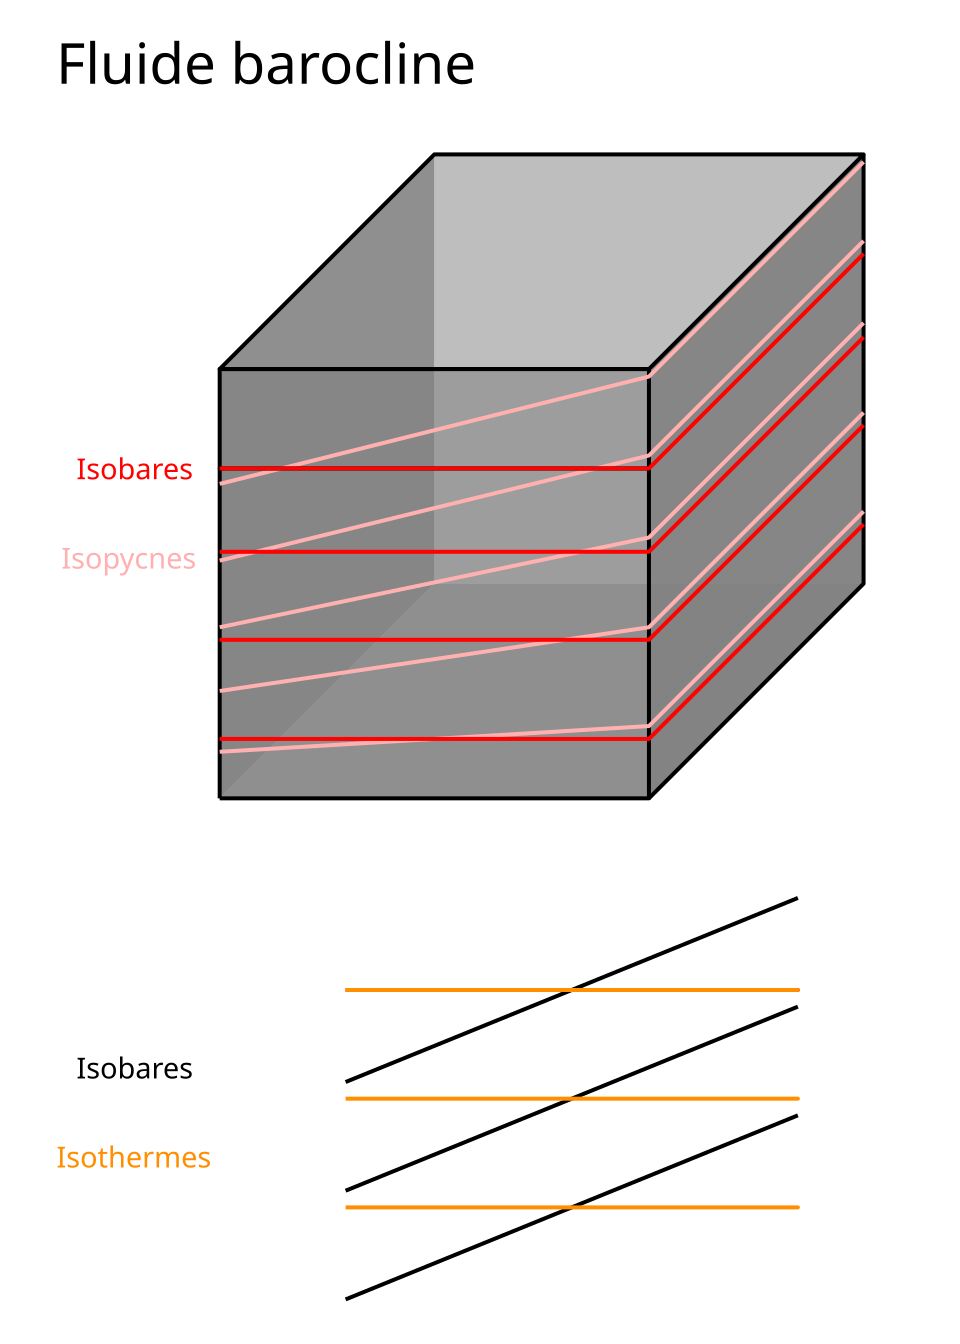
\includegraphics[width=0.3\textwidth]{images/annexes/Baroclinic_Fluid_Diagram_Text.svg}
		\caption{Croisement des niveaux des isobares avec ceux de densité égales (isopycnes) dans la verticale, ou de la température dans l'horizontale}
		\label{fig:baroclinicfluiddiagramtext}
	\end{figure}
	
	
	\subsection{Barotropicité} 
	Un fluide barotrope est un fluide dans lequel les surfaces d'égale pression (isobares) se confondent avec celles d'égale densité (isopycnes). \cite{wikipedia_barotrope}
	\begin{figure}[H]
		\centering
		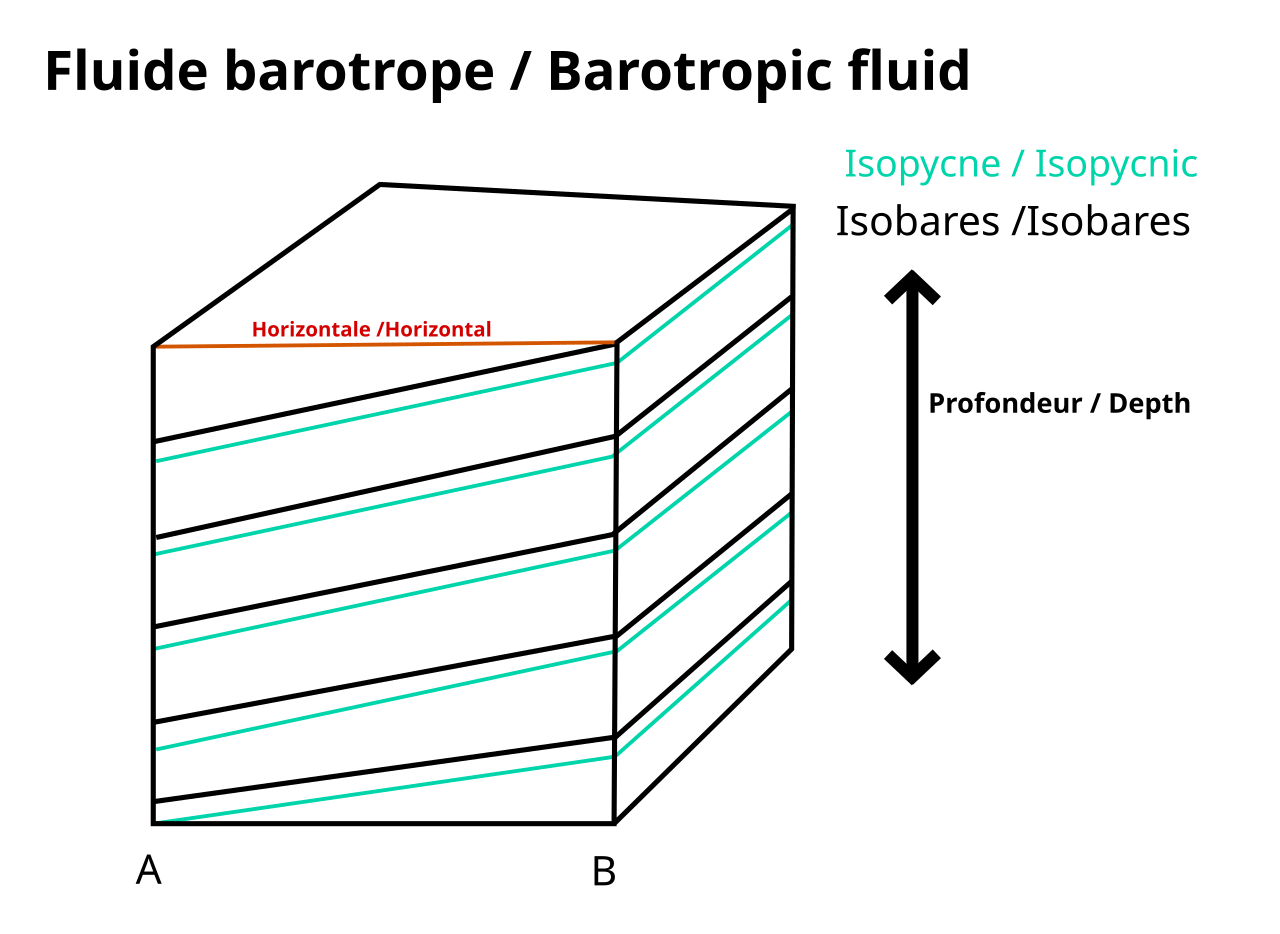
\includegraphics[width=0.3\textwidth]{images/annexes/Barotrope.svg}
		\caption{Stratification des niveaux d'égale pression et d'égale densité dans un fluide barotrope}
		\label{fig:barotrope}
	\end{figure}
	
	\subsection{Thermocline} La thermocline est la zone de transition thermique rapide entre les eaux superficielles de l'océan (généralement plus chaudes et oxygénées) et les eaux profondes (généralement plus froides et anoxiques et parfois plus salées).
	
	Pour la faune, quand elle est très marquée, la thermocline peut être un écotone (zone de transition entre deux écosystèmes), voire jouer le rôle d'une véritable barrière, surtout si elle est associée à une différence forte de salinité, ou à une chute d'oxygène (d'un côté ou de l'autre de la thermocline) \cite{wikipedia_thermocline}
	
	\subsection{Isopycne (Isopycnal)} Une isopycne est une ligne joignant les points de même densité dans un fluide \cite{wikipedia_isopycnal}
	
	\clearpage
	\printbibliography
\end{document}